\documentclass[a4paper, 11pt]{article}

\usepackage{subfiles}

\usepackage[utf8]{inputenc}

\usepackage[
backend=biber,
style=alphabetic,
sorting=ynt
]{biblatex}
 
\addbibresource{bibliography.bib}

\usepackage{textcomp}
\usepackage[T1]{fontenc}
\usepackage{multirow}
\usepackage{float}
\usepackage[caption = false]{subfig}
\usepackage{longtable}
\usepackage{listings}
\usepackage{mathtools}
\DeclareMathOperator{\tr}{Tr}
\usepackage{commath}
\usepackage{bbold}
\usepackage{xcolor}
\usepackage{physics}
%\usepackage[margin=1.8cm]{geometry}

\usepackage{tikz-cd} 
\usepackage{amsmath}
\usepackage{amsfonts}
\usepackage{amssymb}
\usepackage{amsthm}
\usepackage{graphicx}
\usepackage[colorinlistoftodos]{todonotes}
\usepackage[colorlinks=true, allcolors=blue]{hyperref}
\usepackage{siunitx}
\sisetup{separate-uncertainty=true}

\usepackage[sc]{mathpazo}
\linespread{1.05}         % Palladio needs more leading (space between lines)
\usepackage[T1]{fontenc}

\newcommand{\diag}[1]{\text{diag}\qty(#1)}
\newcommand{\Lagr}{\mathcal{L}}
\newcommand{\const}{\text{const}}
\newcommand{\sign}[1]{\text{sign}\qty(#1)}

\title{Relativistic non-ideal flows}
\author{Jacopo Tissino}
\date{2019}

\begin{document}

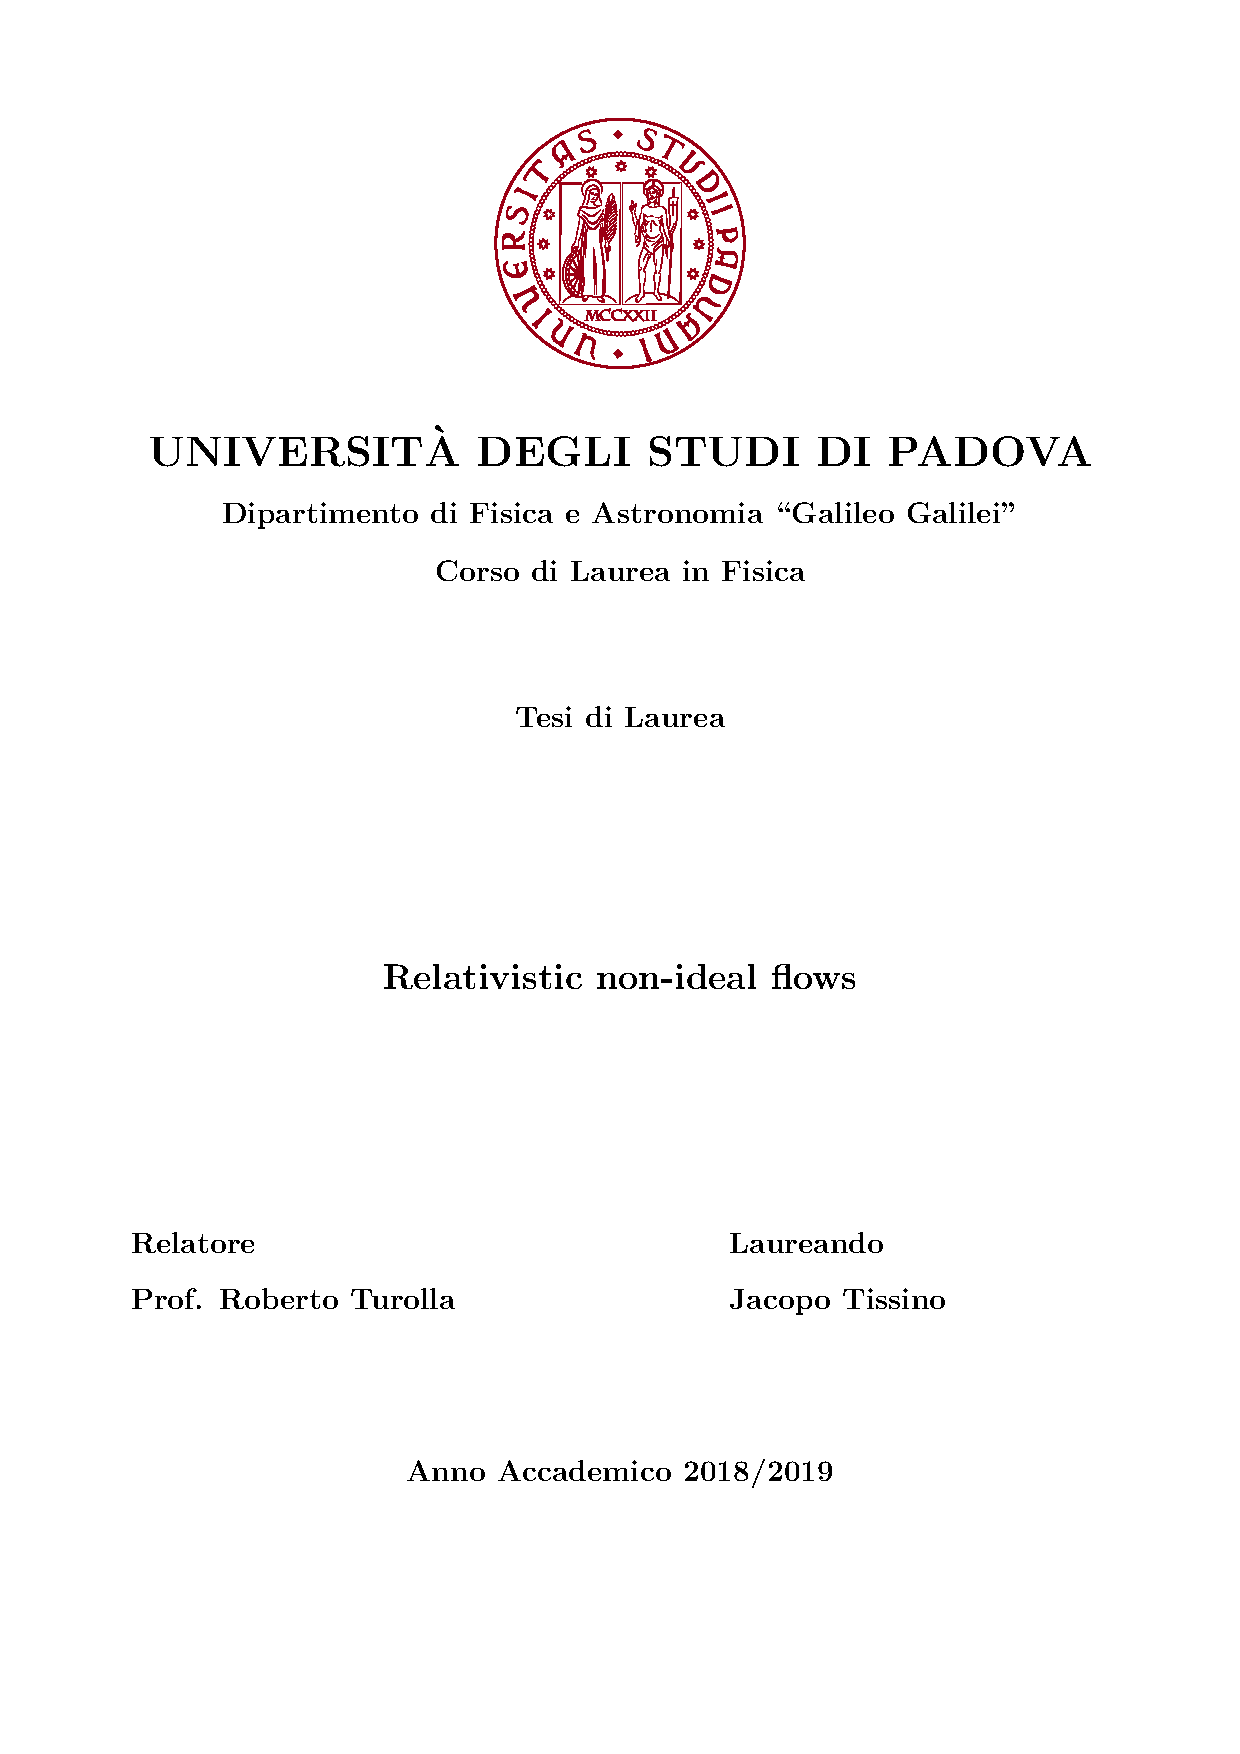
\includepdf[pages=1]{Frontespizio_Laurea.pdf}

\begin{abstract}
After reviewing the basic concepts of general-relativistic fluid mechanics, I will focus on the treatment of non-ideal
(viscous, thermo-conducting) flows. An application of non-ideal relativistic flows to spherical accretion onto black holes
(generalized Bondi accretion) will be also discussed.
\end{abstract}

\setcounter{tocdepth}{4}
\cftsetindents{paragraph}{5em}{0in}
The table of contents will only include up to the subsection level in the final document, it is just convenient for drafts to be able to see the paragraph structure.
\tableofcontents

\section{Notational preface} \label{sec:notational-preface}
\subfile{conventions.tex}

\section{Relativity} \label{sec:general-relativity}
\subfile{general-relativity-basics.tex}

\section{Fluid dynamics} \label{sec:fluid-dynamics}
\subfile{relativistic-fluid-mechanics.tex}

\section{Radiative effects in spherical accretion} \label{sec:radiative-effects}
\subfile{radiative-effects.tex}

% \section{Extra sections, possibly to remove} \label{sec:formulas}
% \subfile{formulas.tex}

\printbibliography[title={Bibliography}]

%\printindex

\end{document}
